\documentclass{standalone}
\usepackage{tikz}
\usetikzlibrary{patterns, positioning}


\begin{document}
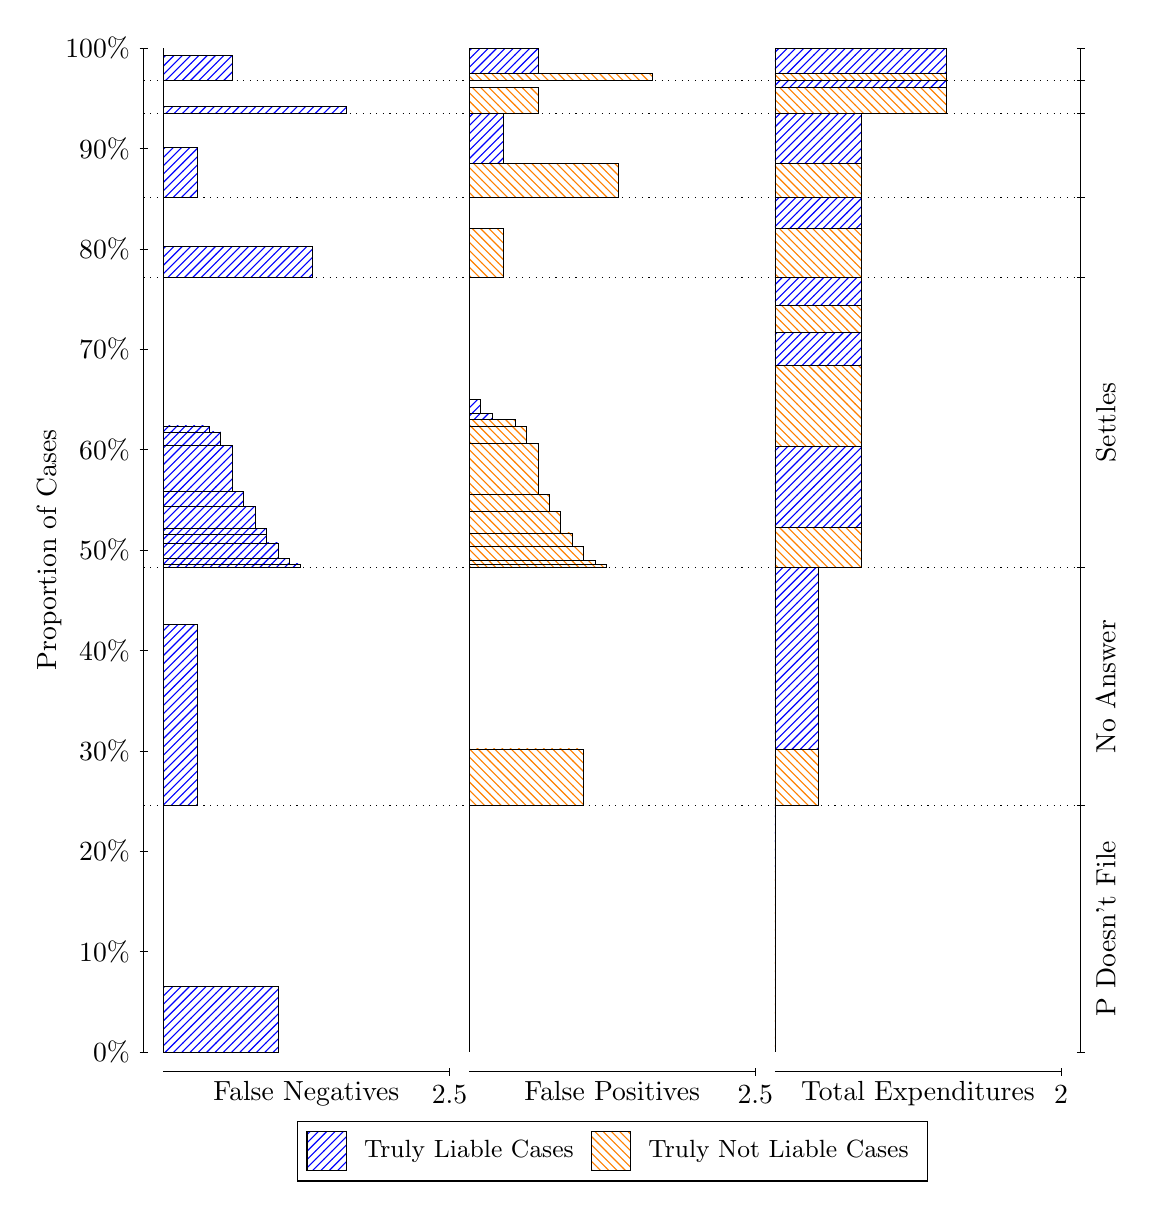
\begin{tikzpicture}
\draw[black, very thin] (1.5,1.75) -- (1.5,14.5);
\node[rotate=90, text=black, anchor=center] at (0.3, 8.125) {Proportion of Cases};
\draw[black, very thin] (1.45,1.75) -- (1.55,1.75);
\node[text=black, anchor=east] at (1.45, 1.75) {0\%};
\draw[black, very thin] (1.45,3.025) -- (1.55,3.025);
\node[text=black, anchor=east] at (1.45, 3.025) {10\%};
\draw[black, very thin] (1.45,4.3) -- (1.55,4.3);
\node[text=black, anchor=east] at (1.45, 4.3) {20\%};
\draw[black, very thin] (1.45,5.575) -- (1.55,5.575);
\node[text=black, anchor=east] at (1.45, 5.575) {30\%};
\draw[black, very thin] (1.45,6.85) -- (1.55,6.85);
\node[text=black, anchor=east] at (1.45, 6.85) {40\%};
\draw[black, very thin] (1.45,8.125) -- (1.55,8.125);
\node[text=black, anchor=east] at (1.45, 8.125) {50\%};
\draw[black, very thin] (1.45,9.4) -- (1.55,9.4);
\node[text=black, anchor=east] at (1.45, 9.4) {60\%};
\draw[black, very thin] (1.45,10.675) -- (1.55,10.675);
\node[text=black, anchor=east] at (1.45, 10.675) {70\%};
\draw[black, very thin] (1.45,11.95) -- (1.55,11.95);
\node[text=black, anchor=east] at (1.45, 11.95) {80\%};
\draw[black, very thin] (1.45,13.225) -- (1.55,13.225);
\node[text=black, anchor=east] at (1.45, 13.225) {90\%};
\draw[black, very thin] (1.45,14.5) -- (1.55,14.5);
\node[text=black, anchor=east] at (1.45, 14.5) {100\%};

\draw[black, very thin] (13.4,1.75) -- (13.4,14.5);
\draw[black, very thin] (13.35,1.75) -- (13.45,1.75);
\node[anchor=west] at (13.35, 1.75) {};
\draw[black, very thin] (13.35,4.8788) -- (13.45,4.8788);
\node[anchor=west] at (13.35, 4.8788) {};
\draw[black, very thin] (13.35,7.9015) -- (13.45,7.9015);
\node[anchor=west] at (13.35, 7.9015) {};
\draw[black, very thin] (13.35,11.587) -- (13.45,11.587);
\node[anchor=west] at (13.35, 11.587) {};
\draw[black, very thin] (13.35,12.604) -- (13.45,12.604);
\node[anchor=west] at (13.35, 12.604) {};
\draw[black, very thin] (13.35,13.668) -- (13.45,13.668);
\node[anchor=west] at (13.35, 13.668) {};
\draw[black, very thin] (13.35,14.086) -- (13.45,14.086);
\node[anchor=west] at (13.35, 14.086) {};
\draw[black, very thin] (13.35,14.5) -- (13.45,14.5);
\node[anchor=west] at (13.35, 14.5) {};

\draw[black, very thin, pattern color=blue, pattern=north east lines] (1.75,1.75) rectangle (3.2033,2.5798);
\draw[black, very thin, pattern color=orange, pattern=north west lines] (1.75,2.5798) rectangle (1.75,4.8788);
\draw[black, very thin, pattern color=blue, pattern=north east lines] (1.75,4.8788) rectangle (2.186,7.1822);
\draw[black, very thin, pattern color=orange, pattern=north west lines] (1.75,7.1822) rectangle (1.75,7.9015);
\draw[black, very thin, pattern color=blue, pattern=north east lines] (1.75,7.9015) rectangle (3.494,7.9485);
\draw[black, very thin, pattern color=blue, pattern=north east lines] (1.75,7.9485) rectangle (3.3487,8.021);
\draw[black, very thin, pattern color=blue, pattern=north east lines] (1.75,8.021) rectangle (3.2033,8.2149);
\draw[black, very thin, pattern color=blue, pattern=north east lines] (1.75,8.2149) rectangle (3.058,8.3205);
\draw[black, very thin, pattern color=blue, pattern=north east lines] (1.75,8.3205) rectangle (3.058,8.4033);
\draw[black, very thin, pattern color=blue, pattern=north east lines] (1.75,8.4033) rectangle (2.9127,8.6745);
\draw[black, very thin, pattern color=blue, pattern=north east lines] (1.75,8.6745) rectangle (2.7673,8.8701);
\draw[black, very thin, pattern color=blue, pattern=north east lines] (1.75,8.8701) rectangle (2.622,9.4516);
\draw[black, very thin, pattern color=blue, pattern=north east lines] (1.75,9.4516) rectangle (2.4767,9.626);
\draw[black, very thin, pattern color=blue, pattern=north east lines] (1.75,9.626) rectangle (2.3313,9.7023);
\draw[black, very thin, pattern color=orange, pattern=north west lines] (1.75,9.7023) rectangle (1.75,11.587);
\draw[black, very thin, pattern color=blue, pattern=north east lines] (1.75,11.587) rectangle (3.6393,11.979);
\draw[black, very thin, pattern color=orange, pattern=north west lines] (1.75,11.979) rectangle (1.75,12.604);
\draw[black, very thin, pattern color=blue, pattern=north east lines] (1.75,12.604) rectangle (2.186,13.238);
\draw[black, very thin, pattern color=orange, pattern=north west lines] (1.75,13.238) rectangle (1.75,13.668);
\draw[black, very thin, pattern color=blue, pattern=north east lines] (1.75,13.668) rectangle (4.0753,13.757);
\draw[black, very thin, pattern color=orange, pattern=north west lines] (1.75,13.757) rectangle (1.75,14.086);
\draw[black, very thin, pattern color=blue, pattern=north east lines] (1.75,14.086) rectangle (2.622,14.411);
\draw[black, very thin, pattern color=orange, pattern=north west lines] (1.75,14.411) rectangle (1.75,14.5);
\draw[black, very thin, pattern color=orange, pattern=north west lines] (5.6333,1.75) rectangle (5.6333,4.049);
\draw[black, very thin, pattern color=blue, pattern=north east lines] (5.6333,4.049) rectangle (5.6333,4.8788);
\draw[black, very thin, pattern color=orange, pattern=north west lines] (5.6333,4.8788) rectangle (7.0867,5.5982);
\draw[black, very thin, pattern color=blue, pattern=north east lines] (5.6333,5.5982) rectangle (5.6333,7.9015);
\draw[black, very thin, pattern color=orange, pattern=north west lines] (5.6333,7.9015) rectangle (7.3773,7.9384);
\draw[black, very thin, pattern color=orange, pattern=north west lines] (5.6333,7.9384) rectangle (7.232,7.995);
\draw[black, very thin, pattern color=orange, pattern=north west lines] (5.6333,7.995) rectangle (7.0867,8.1714);
\draw[black, very thin, pattern color=orange, pattern=north west lines] (5.6333,8.1714) rectangle (6.9413,8.342);
\draw[black, very thin, pattern color=orange, pattern=north west lines] (5.6333,8.342) rectangle (6.796,8.6202);
\draw[black, very thin, pattern color=orange, pattern=north west lines] (5.6333,8.6202) rectangle (6.6507,8.8328);
\draw[black, very thin, pattern color=orange, pattern=north west lines] (5.6333,8.8328) rectangle (6.5053,9.4771);
\draw[black, very thin, pattern color=orange, pattern=north west lines] (5.6333,9.4771) rectangle (6.36,9.692);
\draw[black, very thin, pattern color=orange, pattern=north west lines] (5.6333,9.692) rectangle (6.2147,9.7858);
\draw[black, very thin, pattern color=blue, pattern=north east lines] (5.6333,9.7858) rectangle (5.924,9.862);
\draw[black, very thin, pattern color=blue, pattern=north east lines] (5.6333,9.862) rectangle (5.7787,10.036);
\draw[black, very thin, pattern color=blue, pattern=north east lines] (5.6333,10.036) rectangle (5.6333,11.587);
\draw[black, very thin, pattern color=orange, pattern=north west lines] (5.6333,11.587) rectangle (6.0693,12.211);
\draw[black, very thin, pattern color=blue, pattern=north east lines] (5.6333,12.211) rectangle (5.6333,12.604);
\draw[black, very thin, pattern color=orange, pattern=north west lines] (5.6333,12.604) rectangle (7.5227,13.034);
\draw[black, very thin, pattern color=blue, pattern=north east lines] (5.6333,13.034) rectangle (6.0693,13.668);
\draw[black, very thin, pattern color=orange, pattern=north west lines] (5.6333,13.668) rectangle (6.5053,13.996);
\draw[black, very thin, pattern color=blue, pattern=north east lines] (5.6333,13.996) rectangle (5.6333,14.086);
\draw[black, very thin, pattern color=orange, pattern=north west lines] (5.6333,14.086) rectangle (7.9587,14.175);
\draw[black, very thin, pattern color=blue, pattern=north east lines] (5.6333,14.175) rectangle (6.5053,14.5);
\draw[black, very thin, pattern color=orange, pattern=north west lines] (9.5167,1.75) rectangle (9.5167,4.049);
\draw[black, very thin, pattern color=blue, pattern=north east lines] (9.5167,4.049) rectangle (9.5167,4.8788);
\draw[black, very thin, pattern color=orange, pattern=north west lines] (9.5167,4.8788) rectangle (10.062,5.5982);
\draw[black, very thin, pattern color=blue, pattern=north east lines] (9.5167,5.5982) rectangle (10.062,7.9015);
\draw[black, very thin, pattern color=orange, pattern=north west lines] (9.5167,7.9015) rectangle (10.607,8.4127);
\draw[black, very thin, pattern color=blue, pattern=north east lines] (9.5167,8.4127) rectangle (10.607,9.4399);
\draw[black, very thin, pattern color=orange, pattern=north west lines] (9.5167,9.4399) rectangle (10.607,10.469);
\draw[black, very thin, pattern color=blue, pattern=north east lines] (9.5167,10.469) rectangle (10.607,10.888);
\draw[black, very thin, pattern color=orange, pattern=north west lines] (9.5167,10.888) rectangle (10.607,11.232);
\draw[black, very thin, pattern color=blue, pattern=north east lines] (9.5167,11.232) rectangle (10.607,11.587);
\draw[black, very thin, pattern color=orange, pattern=north west lines] (9.5167,11.587) rectangle (10.607,12.211);
\draw[black, very thin, pattern color=blue, pattern=north east lines] (9.5167,12.211) rectangle (10.607,12.604);
\draw[black, very thin, pattern color=orange, pattern=north west lines] (9.5167,12.604) rectangle (10.607,13.034);
\draw[black, very thin, pattern color=blue, pattern=north east lines] (9.5167,13.034) rectangle (10.607,13.668);
\draw[black, very thin, pattern color=orange, pattern=north west lines] (9.5167,13.668) rectangle (11.697,13.996);
\draw[black, very thin, pattern color=blue, pattern=north east lines] (9.5167,13.996) rectangle (11.697,14.086);
\draw[black, very thin, pattern color=orange, pattern=north west lines] (9.5167,14.086) rectangle (11.697,14.175);
\draw[black, very thin, pattern color=blue, pattern=north east lines] (9.5167,14.175) rectangle (11.697,14.5);
\draw[black, dotted] (1.5,4.8788) -- (13.4,4.8788);
\draw[black, dotted] (1.5,7.9015) -- (13.4,7.9015);
\draw[black, dotted] (1.5,11.587) -- (13.4,11.587);
\draw[black, dotted] (1.5,12.604) -- (13.4,12.604);
\draw[black, dotted] (1.5,13.668) -- (13.4,13.668);
\draw[black, dotted] (1.5,14.086) -- (13.4,14.086);
\draw[black, very thin] (1.75,1.5) -- (5.3833,1.5);
\node[text=black, anchor=north] at (3.5667, 1.5) {False Negatives};
\draw[black, very thin] (5.3833,1.45) -- (5.3833,1.55);
\node[text=black, anchor=north] at (5.3833, 1.45) {2.5};

\draw[black, very thin] (5.6333,1.5) -- (9.2667,1.5);
\node[text=black, anchor=north] at (7.45, 1.5) {False Positives};
\draw[black, very thin] (9.2667,1.45) -- (9.2667,1.55);
\node[text=black, anchor=north] at (9.2667, 1.45) {2.5};

\draw[black, very thin] (9.5167,1.5) -- (13.15,1.5);
\node[text=black, anchor=north] at (11.333, 1.5) {Total Expenditures};
\draw[black, very thin] (13.15,1.45) -- (13.15,1.55);
\node[text=black, anchor=north] at (13.15, 1.45) {2};

\node[text=black, centered, rotate=90] at (13.72, 3.3144) {P Doesn't File};
\node[text=black, centered, rotate=90] at (13.72, 6.3902) {No Answer};
\node[text=black, centered, rotate=90] at (13.72, 9.744) {Settles};





\draw (7.449999999999999,1.5) node[draw=none] (baseCoordinate) {};
\begin{scope}[align=center]
        \matrix[scale=0.5, draw=black, below=0.5cm of baseCoordinate, nodes={draw}, column sep=0.1cm]{
            \node[rectangle, draw, minimum width=0.5cm, minimum height=0.5cm, pattern color=blue, pattern=north east lines] {}; &
            \node[draw=none, font=\small, text=black] (B) {Truly Liable Cases}; &
            \node[rectangle, draw, minimum width=0.5cm, minimum height=0.5cm, pattern color=orange, pattern=north west lines] {}; &
            \node[draw=none, font=\small, text=black] (B) {Truly Not Liable Cases}; \\
            };
\end{scope}

\end{tikzpicture}
\end{document}